%!TEX program = xelatex
%%%%%%%%%%%%%%%%%%%%%%%这是导言部分的开始%%%%%%%%

%========= 导言部分声明文档的类型=================
\documentclass{article}

	%=========导言部分可可以加载宏包=================
	\usepackage{amsmath}                % 数学公式排版宏包
	\usepackage{amssymb}                % 数学符号命令宏包
	\usepackage{amsthm}                 % 数学定理宏包
	\usepackage[UTF8]{ctex}             % 中文输入宏包
	\usepackage[a4paper]{geometry}      % 页面设置宏包
	\usepackage{setspace}               % 行间距宏包
	\usepackage{graphicx}               % 图片宏包
	\usepackage{listings}               % 代码宏包
	\usepackage{color}					% 颜色宏包
	\usepackage{xcolor}                 % 颜色处理宏包
	\usepackage{float}                  % 浮动对象式样宏包
	\usepackage{fontspec}
	\usepackage{enumerate}				% 列举编号包
	
	%=========页面设置==============================
	\geometry{left=1cm,right=1cm,top=1cm,bottom=2cm}
	\onehalfspacing
	\setlength\parindent{0em}

	%=========代码格式设置============================
	\definecolor{dkgreen}{rgb}{0,0.6,0}
	\definecolor{gray}{rgb}{0.5,0.5,0.5}
	\definecolor{mauve}{rgb}{0.58,0,0.82}
	% \setmonofont{Consolas}
	\lstset{
		numbers = left, 	
		numberstyle = \color{gray}, 
		keywordstyle = \color{blue},
		commentstyle = \color{dkgreen}, 
		stringstyle = \color{mauve},
		basicstyle = \ttfamily,
		breaklines = true,
		frame = shadowbox, % 阴影效果
		rulesepcolor = \color{ red!20!green!20!blue!20} ,
		escapeinside = ``, % 英文分号中可写入中文
		xleftmargin = 2em,xrightmargin=2em, aboveskip=1em,
		framexleftmargin = 2em
	} 

%=========导言部分可以定义标题信息===============
\title{组会报告}
\author{徐益}
\date{\today}
%%%%%%%%%%%%%%%%%%%%%%%这是导言部分的结束%%%%%%%%%

%%%%%%%%%%%%%%%%%%%%%%%这是正文部分的开始%%%%%%%%%
\begin{document}

%=========生成标题================================
\maketitle

%=========开始正文的输入==========================

%===========第一节=================
\section{工作内容}
1. 数据采集测试;

% 2. 修改仿真报告;

% 3. 学习LDPC低时延译码方案。

%===========第一节=================
\section{数据采集测试}
\subsection{ramdisk}
\subsubsection{传统ramdisk}
% \lstset{language=C++}
\begin{lstlisting}
# mkdir /mnt/test
# mke2fs /dev/ram0
# mount /dev/ram /mnt/test
\end{lstlisting}
写入速率:700MB/s~800MB/s
\subsubsection{ramfs}
\begin{lstlisting}
# mkdir /testRam
# mount -t ramfs none /testRAM
# mount -t ramfs none /testRAM -o maxsize=2000
\end{lstlisting}
写入速率:900MB/s~1100MB/s
\subsubsection{tmpfs}
\begin{lstlisting}
# mkdir -p /mnt/tmpfs
# mount tmpfs /mnt/tmpfs -t tmpfs
# mount tmpfs /mnt/tmpfs -t tmpfs -o size=32g
\end{lstlisting}
写入速率:1.2GB/s~1.3GB/s

\subsection{测试结果}
\begin{figure}[H]
	\centering
	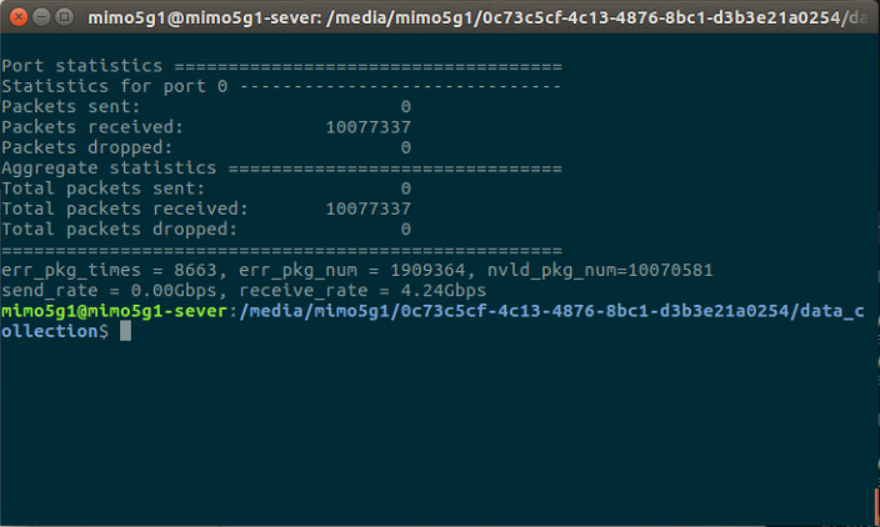
\includegraphics[width = .8\textwidth]{res5ssd.png}
	\caption{向ssd写入}
\end{figure}
\begin{figure}[H]
	\centering
	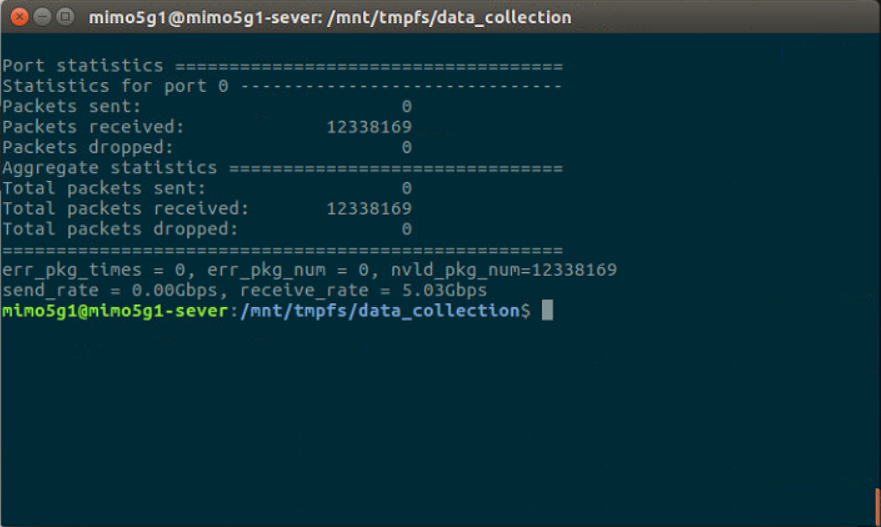
\includegraphics[width = .8\textwidth]{res5ram.png}
	\caption{向tempfs写入}
\end{figure}

%===========第三节=================
% \section{学习LDPC低时延译码方案}
% \begin{figure}[H]
% 	\centering
% 	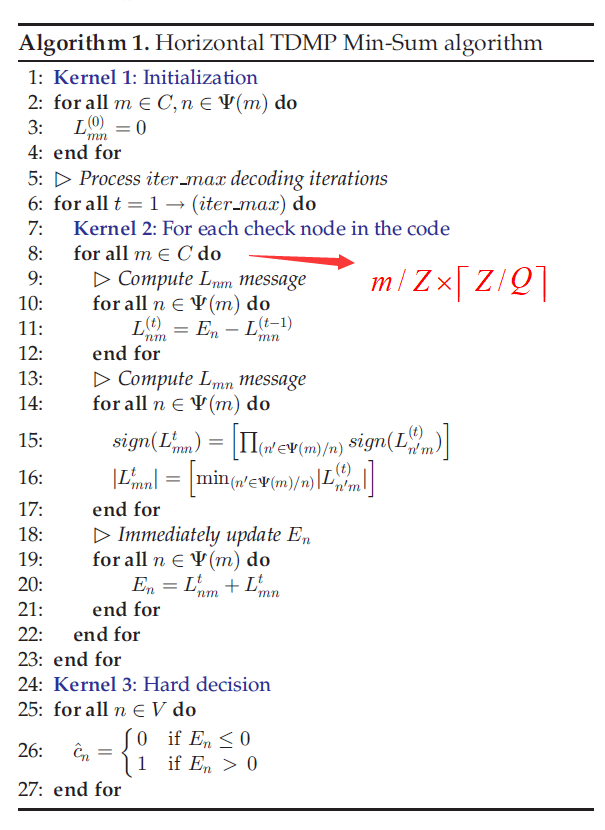
\includegraphics[width = .8\textwidth]{al.png}
% 	\caption{原算法}
% \end{figure}
% 两个问题:\\
% 1. the processor has Q SIMD processing units whereas QC-LDPC 
% code has a Z CN structure organization;\\
% 若$Q=32,Z=42$,则利用率为$42/64$。
% \begin{figure}[H]
% 	\centering
% 	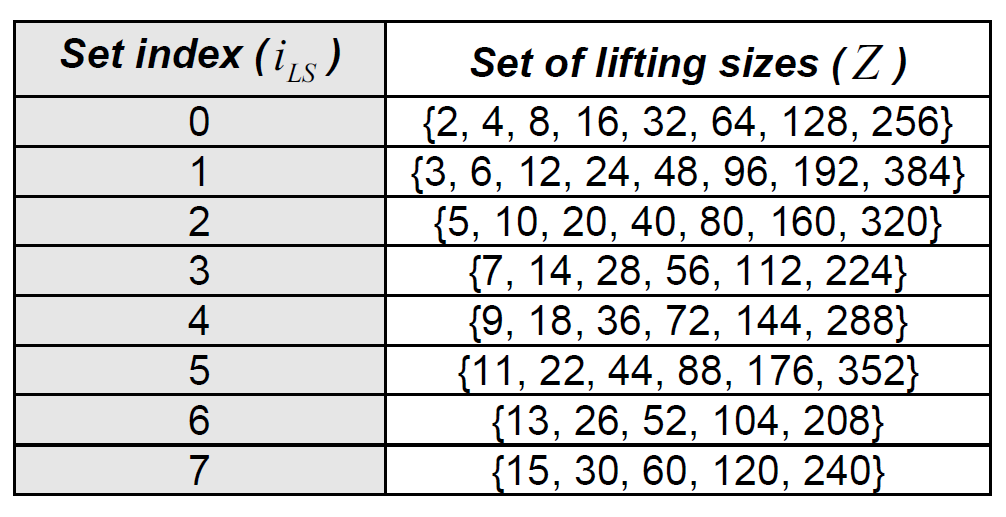
\includegraphics[width = .6\textwidth]{zc.png}
% 	\caption{5GNRZc取值}
% \end{figure}
% 2. SIMD logical rotate feature and scatter \& gather memory 
% operations are unavailable to access to the Z VN elements.\\
% \begin{figure}[H]
% 	\centering
% 	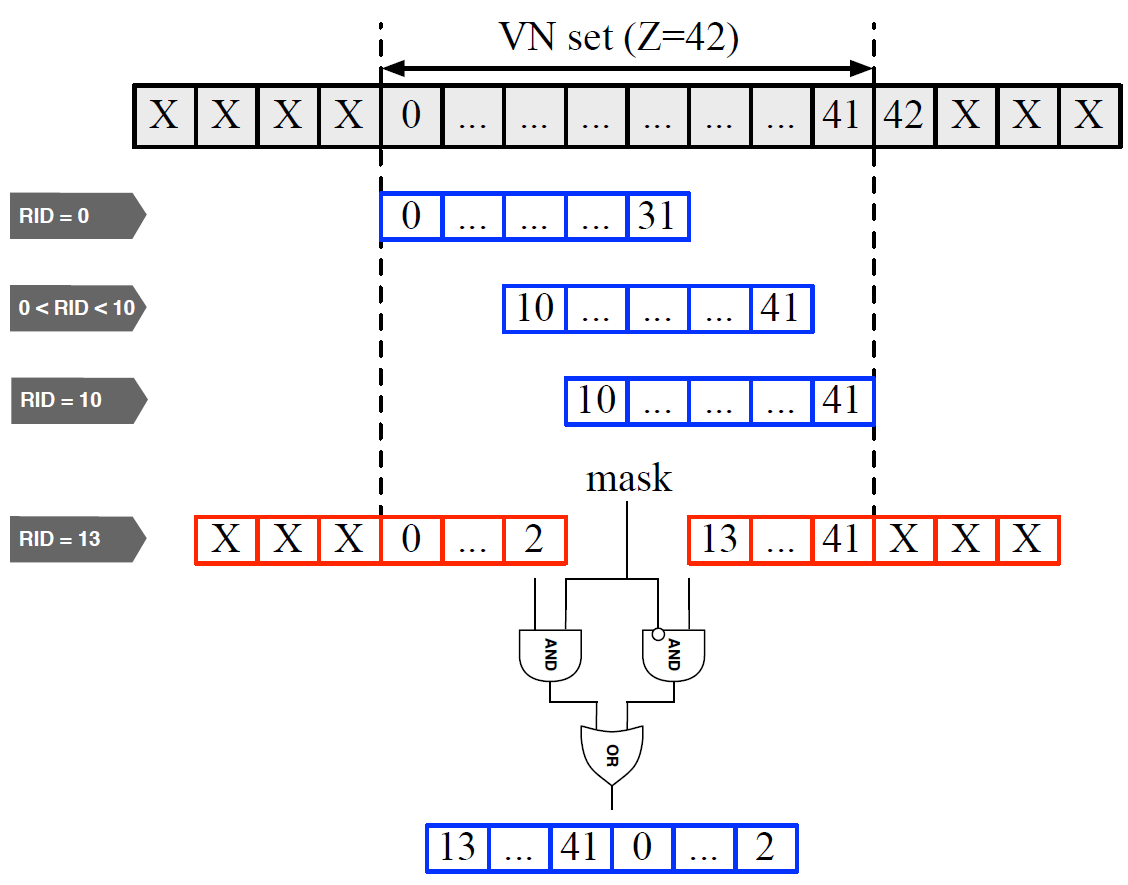
\includegraphics[width = .8\textwidth]{vn.png}
% 	\caption{VN接入方式($Z_c=42,Q=32$)}
% \end{figure}


%===========第二节=================
% \section{改写仿真报告}
%===========第四节=================
% \section{仍存在的问题}


%===========下周计划=================
% \section{下阶段计划}
% 1. 继续完成仿真报告

\end{document}
%%%%%%%%%%%%%%%%%%%%%%%这是正文部分的结束%%%%%%%%%%%%